\chapter{Background \& Objectives}

%This section should discuss your preparation for the project, including background reading, your analysis of the problem and the process or method you have followed to help structure your work.  It is likely that you will reuse part of your outline project specification, but at this point in the project you should have more to talk about.

%\textbf{Note}:

%\begin{itemize}
   %\item All of the sections and text in this example are for illustration purposes. The main Chapters are a good starting point, but the content and actual sections that you include are likely to be different.

  % \item Look at the document on the Structure of the Final Report for additional guidance.

%\end {itemize}

\section{Background}
%What was your background preparation for the project? What similar systems did you assess? What was your motivation and interest in this project?
Handwriting notes is still considered to be an important aspect of note taking. Smoker et al \cite{citeulike:13988059} conducted a study comparing handwritten text against digital text for memory retention and out of 61 adults 72.1\% prefered to take notes using pen and paper, rather than on a computer. Smoker et al concluded that recall rates for handwritten text was greater than that of typed text proving that handwritten notes are better for a user's memory retention.

However technology has advanced and we're moving into an era where we track and view everything digitally, from email to calendar entries. Therefore, there is a need to transfer the productivity from handwritten notes to digital notes - so they can be located easily.

% Handwriting triaining ?

% Taxonomy of notes 
When a user creates a note they will often come in differing forms: some are semi-structured and some are back of the evenvelope kind of notes. When thinking about an application to analyse notes, first there has to be consideration for what a note will consist of. A taxonomy, by definition, is a biological term for a classification of similar sections, showing how things are linked together. 

Notes can be throught of as a collection of similar classifications, whether this is the pure textual descriptions of a note or whether this is purely pictoral form or a mixture of both. However, the notes are normally split into three distinct categories: 
\begin{enumerate}
	\item Textual descriptions
	\item Diagrams 
	\item Graphs
\end{enumerate}
\begin{figure}[h!]
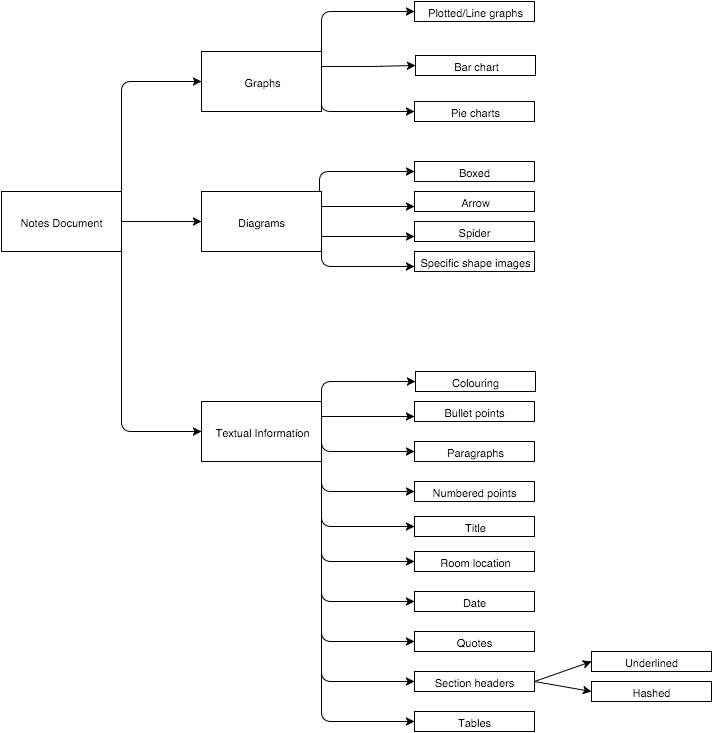
\includegraphics[scale=0.5]{images/taxonomy}
\centering
\caption{A taxonomy showing the structure and classification of different types of notes and what is contained in a note.}
 \label{fig:taxonomyofnotes}
\end{figure}

In figure \ref{fig:taxonomyofnotes}, it shows a taxonomy of the different aspects which may comprise to make a note. Textural descriptions form the core part of a note, this is essentially the important content that a note-taker is trying to remember and write down. Different note-takers form their notes in different ways, for example the headings may be underlined or hashed - if they were adopting a mark-down style approach. These sections helps to show that there's a break in the content, and should be sub-sectioned. Textural points that are short, but important, are often characterised by a colon or a bullet point; these are the most common form of concise note building, in the classisifcation. Coloured highlighting if often used for a variety of reasons: it stands out on the page and for some people colour retention is better. Finally, tables help to represent textual content in tabular form.  This is often good in notes for comparisons. 

Graphs are great visual tools for user's in helping to convery textual information in a graphical form. Naturally, they have their limitations such as they come in different shapes and sizes, such as a line-graph, pie chart or a bar chart. Coupled with graphs, notes often consist of diagram drawings.  In figure \ref{fig:taxonomyofnotes}, there are different sections and classsifications of a diagram: boxed, arrow etc. Each one has its own purpose and arrowed and box can overlap; UML diagrams are a case of this. Spider diagrams are probably the hardest to represent, due to the varying sizes and whether the user draws circles or clouds. Furthermore, specific shape diagrams are conceptutally hard to think about as it depends on the domain in which the user is drawing the note. For example, a person in biology may draw a stick person, whereas someone in Computer Science may draw a PC. 

Overall, identifying the taxonomy of notes is important as it gives context to which the application can potentially parse and identify these different classifications. Additionally, it acknowledges where there may need to be constraints due to the variations in notes and how it can deal with semi-structured documents.

% Add some more from the stuff Hannah made us write about in the first week.



\subsection{Similar Systems}
There are a number of systems which offer similar, and sometimes the same functionality that MapMyNotesApplication would use. The systems are
\begin{itemize}
  \item OneNote
  \item EverNote
\end{itemize}
Each of these tools offer something slightly different and it would be good to produce a system that would encapse these different aspects.
\subsubsection{OneNote}
OneNote is a note-taking and organisational app made by Microsoft [cite].
\subsubsection{EverNote}
EverNote is a note-taking and note organisation app, it is both supported on the web and in app form. EverNote is widely used and would provide a lot of the functionality a user would need to upload their note. They have realeased development articles [CITE-2013 one] stating that they are able to do OCR recognition on images. This would allow the user to upload an image and it would give a list of words, which it thinks is the word identified. This differs from MapMyNotes where the author aims to develop an application which would give a 1-1 word comparision, rather than a list of words.


\subsection{Why this project?}
The author's motivation for this project is to provide a tool, which initially would be tailored to lecturer based note content. Often notes are written up, but discarded into a big pile and later they're hard to find. As a user, it would be good if the notes were all in one place that they could photograph in and it would automatically create meta-data for it and save it to their calendar. Often the modules that are undertaken are stored in my calendar as a reminder that there's a lecturer on that day - so providing a link to the event in the calendar would be a nice way to tie all these dispersed information together.

\section{Analysis}
%Taking into account the problem and what you learned from the background work, what was your analysis of the problem? How did your analysis help to decompose the problem into the main tasks that you would undertake? Were there alternative approaches? Why did you choose one approach compared to the alternatives?

%There should be a clear statement of the objectives of the work, which you will evaluate at the end of the work.

%In most cases, the agreed objectives or requirements will be the result of a compromise between what would ideally have been produced and what was felt to be possible in the time available. A discussion of the process of arriving at the final list is usually appropriate.
By analysing the problem a taxonomy of notes was collated. This helped to breakdown exactly what was in a set of notes. This taxonomy gave a comprehensive analysis of what information would be available to parse from the test, as well as giving the information parsed semantic meaning. It was quickly brought up that I should potentially create a specific layout for the note so that the data can be parsed sensibly, to reduce the complexity.

After identifying that handwriting recognition would be a part of the application then research began investigating what OCR (optical character recognition) tools are available. It was suggested that the open source tool Tesseract [cite] would be an appropriate tool. Instead of using an OCR tool then I could have focussed my dissertation on analysing notes and extracting user's handwriting from it - however, that is not within the aim of the project. As it is more of a tool to use, then using an OCR eases the complexity.

The main objective of the tool would allow a user to upload a photo of their handwritten notes. It will use very basic OCR analysis of meta-data such as the date, lecturer, module code, lecture title and location from the user's handwriting. For the very basic application the handwriting would analyse the author's handwriting. The application will be able to add and edit meta-data relating to a note they upload to the web application. The user will then be able to search for a given module code, they would then be expected to view their notes that they have made. Futhermore, they would be expected to be able to view all the notes that they have entered into the application.

With the web application, it is expected that the user will be able to integrate with their calendar. Google Calendar has been chosen for the calendar the application will interact with. This would have to interact via oAuth. The calendar would be integrated when the user views the homepage to see all their notes, and when they save the note it will update a calendar event of the given day - adding the note URL.

Ideally, there would be more features available in the release but due to the time constraints then certain functionality was not in the primary goals. Analysing the whole note and converting it all to text and displaying the appropriate colour from the note would have been a nice feature to have and would have been really useful. However, this is far too complex within the timeframe that was available. Instead the parsing of the meta-data would be considered enough instead of this additional feature.

During the first few meetings my supervisor, Dr Hannah Dee, it was discussed what was actually plausable in the time frame. Acknowledging that the project was large and could be expanded we opted to rein in the features and get a minimal project. Dr Hannah Dee suggested that the just the application without the Tesseract parsing would be enough for a minimal product, however I wanted the ability to try and recognise handwriting recognition. So we comprised but mentioned that the handwriting recognition would be a background process, and not the main aim.


\begin{itemize}
  \item Looked into different ways to binarise an image accordingly.
  \item Created a list of user stories after the discussion with hannah to decompose the problems.
  \item I chose to do OCR recognition for singular pages and hopefully getting th etop 3 lines as meta-data than normal notes because I needed structure.
\end{itemize}

\section{Process}
%You need to describe briefly the life cycle model or research method that you used. You do not need to write about all of the different process models that you are aware of. Focus on the process model that you have used. It is possible that you needed to adapt an existing process model to suit your project; clearly identify what you used and how you adapted it for your needs.
Due to the flexibility and the unknown nature of certain aspects of the project, such as how long handwriting training and the calendar integration would take, then a normal plan-driven approach like the waterfall approach would not be suitable. Therefore, due to the changing nature of the project it was agreed that an Agile Metholodoly approach was to be followed.

The chosen Agile Metholodgy was Scrum. This was coupled with principles from Extreme Programming, such as: merciless refactoring and continuous integration. In a Scrum approach work is split into sprints, which define what should be done that week. These normally consist of user stories such as: \textit{As a user I want to be able to search for a given module, so that I can find all notes for that module}. This story is used as a reminder for some feature value. The story is then split into tasks which act as acceptance criteria for the story - this acceptance criteria is used to evaluate the story once it's completed to make sure that it's fully completed.

Once the acceptance critera has been specified I estimate the complexity of that task, in comparision to a ``goldilock'' task.  For my planning I adpated the planning poker technique - where the task goes from 1, 2, 3, 5, 8 and so on. Normally, if I got to the 15 mark then I felt the story was too large and needed to be reviewed and broke down, and the process would start again.

At the end of the sprint a review and restrospected was conducted, this was in the form of a blog post instead of a group, and the primary aims of this was to analyse performance and how I could improve over the next sprint. The retrospectives were key to highlighting issues as well as reflecting on what went well, so I can improve the process and the work produced.

Choosing story points per sprint was not just pot luck or what the customer, in this case the supervisor, wanted the most. At the end of every sprint a tally was kept of how many story points were completed, this would then be brought forward to the next sprint as how many story points should be completed that week. For example, if you completed 20 story points one week your next weeks estimation would be 20 story points worth.


\begin{itemize}
  \item Taiga.io
\end{itemize}
In addition to Scrum the process has been modified to incorporate Extreme Programming principles. They involved test-driven-development, so the tests were written first to give me a better understanding of the underlying design. This coupled with the constant mericless refactoring allowed me to have confidence in the system I was building would still pass the appropriate tests. Furthermore, continuous integration tools were used on the project. TravisCI was used [CITE] and although it's normally for teams, it was good for the build automation and to ensure code was being plaed in the repository. Finally, CRC were used appropriately when thinking about how the classes interacted with one another - this was another way to help and think about the design of the application.
